\documentclass{article}
\usepackage{tikz}
\usetikzlibrary{bayesnet}

\begin{document}
\section{Factor Graph for X-Coordinates}
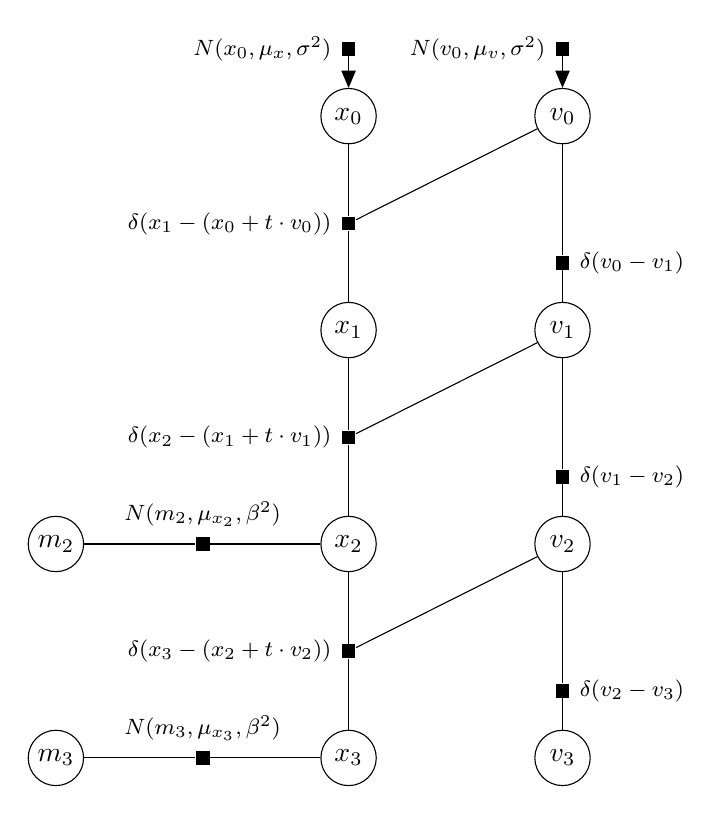
\begin{tikzpicture}
  % Nodes
  \node[latent] (x0) {$x_0$};
  \node[latent, below=of x0, yshift=-1cm] (x1) {$x_1$};
  \node[latent, below=of x1, yshift=-1cm] (x2) {$x_2$};
  \node[latent, below=of x2, yshift=-1cm] (x3) {$x_3$};

  \node[latent, right=of x0, xshift=1cm] (v0) {$v_0$};
  \node[latent, right=of x1, xshift=1cm] (v1) {$v_1$};
  \node[latent, right=of x2, xshift=1cm] (v2) {$v_2$};
  \node[latent, right=of x3, xshift=1cm] (v3) {$v_3$};

  \node[latent, left=of x2, xshift=-2cm] (xo2) {$m_2$};
  \node[latent, left=of x3, xshift=-2cm] (xo3) {$m_3$};

  % Factors
  \factor[above=of x0] {f1} {left:$N(x_0, \mu_{x}, \sigma^2)$} {} {x0};
  \factor[above=of v0] {f2} {left:$N(v_0, \mu_v, \sigma^2)$} {} {v0};
  
  \factor[left=of x2, xshift=-1cm] {f9} {above:$N(m_2, \mu_{x_2}, \beta^2)$} {x2, xo2} {};
  \factor[left=of x3, xshift=-1cm] {f10} {above:$N(m_3, \mu_{x_3}, \beta^2)$} {x3, xo3} {};
  
  \factor[above=of x1, yshift=0.5cm] {f3} {left:$\delta(x_1 - (x_0+t\cdot v_0))$} {x0,x1,v0} {}; %$ N(x_1, x_0+t\cdot v_0, \sigma^2)$
  \factor[above=of x2, yshift=0.5cm] {f4} {left:$\delta(x_2 - (x_1+t\cdot v_1))$} {x1,x2,v1} {}; % $N(x_2, x_1+t\cdot v_1, \sigma^2)$
  \factor[above=of x3, yshift=0.5cm] {f5} {left:$\delta(x_3 - (x_2+t\cdot v_2))$} {x2,x3,v2} {}; % $N(x_3, x_2+t\cdot v_2, \sigma^2)$

  \factor[above=of v1] {f6} {right:$\delta(v_0-v_1)$} {v0,v1} {};
  \factor[above=of v2] {f7} {right:$\delta(v_1-v_2)$} {v1,v2} {};
  \factor[above=of v3] {f8} {right:$\delta(v_2-v_3)$} {v2,v3} {};

\end{tikzpicture}

\vspace{2cm}
\section{New Factor for Y-Coordinates}
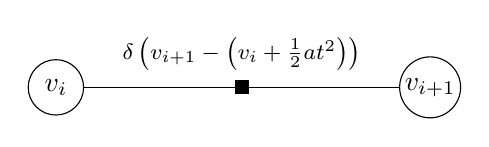
\begin{tikzpicture}

    % Nodes
    \node[latent] (vi) at (0,0) {$v_i$};
    \node[latent, right=4cm of vi] (v1) {$v_{i+1}$};

    \factor[left=of v1, xshift=-1.5cm] {f9} {above:$\delta\left(v_{i+1} - \left(v_i + \frac{1}{2} a t^2\right)\right)$} {vi, v1} {};

\end{tikzpicture}

\end{document}
